% Version: $Revision$

%%%%%%%%%
% Tools %
%%%%%%%%%
\chapter{Tools}
ADAMS, like any other complex project, is using a revision control system to
keep track of changes in the code and a build system to turn the source code
into executable code.

The requirements are as follows:
\begin{tight_itemize}
  \item Java 1.8+
  \item Maven 3.0+
  \item TexLive 2010+ (for compiling the LaTeX documentation)
\end{tight_itemize}

The following sections cover the various tools and environments that are
used when developing for/with ADAMS.

\section{Subversion}
The revision control system that ADAMS uses as backend is Apache Subversion
\cite{subversion}. The ADAMS repository is accessible via the
following URL:

\url{https://svn.cms.waikato.ac.nz/svn/adams/base/trunk/}{}

\noindent You can check out the code in the console using the following
command, provided you have subversion command-line tools installed:
\begin{verbatim}
  svn checkout https://svn.cms.waikato.ac.nz/svn/adams/base/trunk adams
\end{verbatim}

Further modules are available from these repositories:
\begin{tight_itemize}
	\item \textbf{addons} (less common used modules) \\
	\url{https://svn.cms.waikato.ac.nz/svn/adams/addons/trunk/}{}
	\item \textbf{incubator} (experimental modules) \\
	\url{https://svn.cms.waikato.ac.nz/svn/adams/incubator/trunk/}{}
\end{tight_itemize}

\noindent There are lots of graphical clients for subversion available,
open-source and closed-source ones alike. A good overview is accesible through
WikiPedia, \textit{Comparison of Subversion clients}:

\url{http://en.wikipedia.org/wiki/Comparison_of_Subversion_clients}{}

\section{Maven}
ADAMS was designed to be a modular framework, but not only \textit{multi-module}
but \textit{multi-project} and each of the projects consisting of multiple
modules. In order to manage such a complex setup, a build system that can handle
all this was necessary. Apache Maven \cite{maven} fits the bill quite well,
coming with a huge variety of available plug-ins that perform many of the tasks
that are necessary for build management, e.g., generating binary and source code
archives, automatic generation of documentation.

\subsection{Nexus repository manager}
By default, maven merely uses a remote site that one copies archives via
\texttt{scp} or \texttt{sftp}. This approach does not offer a
fine-grained access control, you either have access or you don't. Also, if you
are deploying snapshots on a constant basis, these will start to clutter your
server hosting the archives, since none of them will ever get removed - even
if they are completely obsolete. For better management of the maven repository,
Sonatype's Nexus repository manager \cite{nexus} is used.

In addition to hosting the ADAMS artifacts, Nexus also functions as a proxy to
common maven repositories like Maven Central, JBoss Public, java.net, Codehaus,
Apache and Google Code.

The manager instance for ADAMS is accessible under the following URL:
\url{https://adams.cms.waikato.ac.nz/nexus/}{}

\subsection{Configuring Maven}
In order to gain access to the repositories hosted by the Nexus repository
manager, maven needs to be configured properly. The following steps guide you
through the process:

\heading{Create maven home directory}
First, you need to create maven's home directory, if it doesn't exist already.
The directory is usually located in your home directory and is called
\texttt{.m2}. The full path, on Unix/Linux/Mac systems, is as follows:
\begin{verbatim}
  $HOME/.m2
\end{verbatim}
On Windows, use the following instead:
\begin{verbatim}
  %USERPROFILE\.m2%
\end{verbatim}

\heading{Configure maven}
Download the following configuration file and place it in your maven home directory that you just created:

{\scriptsize \url{https://adams.cms.waikato.ac.nz/resources/settings.xml}{}}

\noindent This file will point maven to ADAMS' repository manager, which manages not only all
the ADAMS modules, but also all its dependencies. It specifies a range of public
repositories, like Maven Central.

\heading{Proxy}
If you are behind a proxy, you need to tell Maven about it. Let's assume that 
your proxy is called \textit{proxy.blah.com} and its port is \textit{3128}.

If you don't need a password to connect to it, you have to add the 
following tag to your \textit{settings.xml} file:
\begin{verbatim}
  <proxies>
    <proxy>
      <active>true</active>
      <protocol>http</protocol>
      <host>proxy.blah.com</host>
      <port>3128</port>
      <nonProxyHosts>localhost|*.blah.com</nonProxyHosts>
    </proxy>
  </proxies>
\end{verbatim}

If your proxy requires a user/password, then you have to 1) generate a master 
password with Maven (which gets stored in \textit{settings-security.xml} in your
Maven home directory) and then 2) the actual password for the proxy. The details are explained 
on the Maven homepage\footnote{\url{http://maven.apache.org/guides/mini/guide-encryption.html}{}}. 
Once you've created the passwords, you have to add the following tag to 
your \textit{settings.xml} file and replace the \textit{USER} and 
\textit{ENCRYPTED\_PASSWORD} placeholders accordingly:
\begin{verbatim}
  <proxies>
    <proxy>
      <active>true</active>
      <protocol>http</protocol>
      <host>proxy.blah.com</host>
      <port>3128</port>
      <username>USER</username>
      <password>{ENCRYPTED_PASSWORD}</password>
      <nonProxyHosts>localhost|*.blah.com</nonProxyHosts>
    </proxy>
  </proxies>
\end{verbatim}

\subsection{Common commands}
Here are a few common maven commands, if you obtained ADAMS from subversion:
\begin{tight_itemize}
	\item Removing all previously generated output: \\
    \texttt{mvn clean}
	\item Compiling the code: \\
    \texttt{mvn compile}
	\item Executing the junit tests: \\
    \texttt{mvn test}
	\item Executing a specific junit test: \\
    \texttt{mvn test -Dtest=<class.name.of.test>}
	\item Packaging up everything: \\
    \texttt{mvn package}
	\item Installing the ADAMS jars in your local maven repository (that will also
	run the tests): \\
    \texttt{mvn install}
	\item You can skip the junit test execution (when packaging or installing) by
	adding the following option to the maven command-line: \\
    \texttt{-DskipTests=true}
\end{tight_itemize}

\subsection{3rd-party libraries}
Make sure that libraries that you use are publicly available from Maven 
Central, \url{http://search.maven.org/}{}, otherwise they won't be considered.

\subsection{Troubleshooting}
\begin{tight_itemize}
  \item \texttt{SSL handshake alert: unrecognized\_name} -- this error occurs starting with Java 7 (or 1.7.0). You can avoid this by setting the \texttt{JAVA\_TOOL\_OPTIONS} environment variable with the following value:
  \begin{verbatim}
  -Djsse.enableSNIExtension=false
  \end{verbatim}
  On Linux or Mac OSX, you would place the following command in your \texttt{\$HOME/.profile} file (effective after logging out and back in again):
  \begin{verbatim}
  export JAVA_TOOL_OPTIONS="-Djsse.enableSNIExtension=false"
  \end{verbatim}
  You can see whether this is set correctly, when Maven reports the following just after issuing a \texttt{mvn} command on command-line:
  \begin{verbatim}
  Picked up JAVA_TOOL_OPTIONS: -Djsse.enableSNIExtension=false
  \end{verbatim}
\end{tight_itemize}

\clearpage
\section{IntelliJ IDEA}
IntelliJ IDEA\cite{intellij} is a light-weight, but very powerful integrated
development environment (IDE), developed by JetBrains\footnote{\url{https://www.jetbrains.com/}{}}.

\subsection{Plug-ins}
The community edition of IntelliJ IDEA (version 14 at time of writing) already
comes bundled with all the necessary plugins for ADAMS development. You only
need to set up ADAMS.

\subsection{Setting up ADAMS}
You can import ADAMS using the start screen of IntelliJ by clicking on
\textit{Import project} as seen in Figure \ref{intellij-import_project-adams2}.
\begin{figure}[htb]
  \centering
  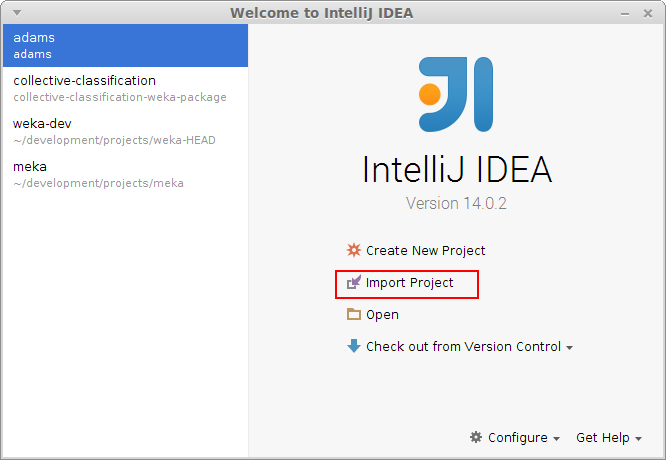
\includegraphics[width=10.0cm]{images/intellij-import_project-adams2.png}
  \caption{IDEA: Importing ADAMS a project.}
  \label{intellij-import_project-adams2}
\end{figure}

Or by selecting \textit{File -> Import project...} from the main menu (see
Figure \ref{intellij-import_project-adams2}).
\begin{figure}[htb]
  \centering
  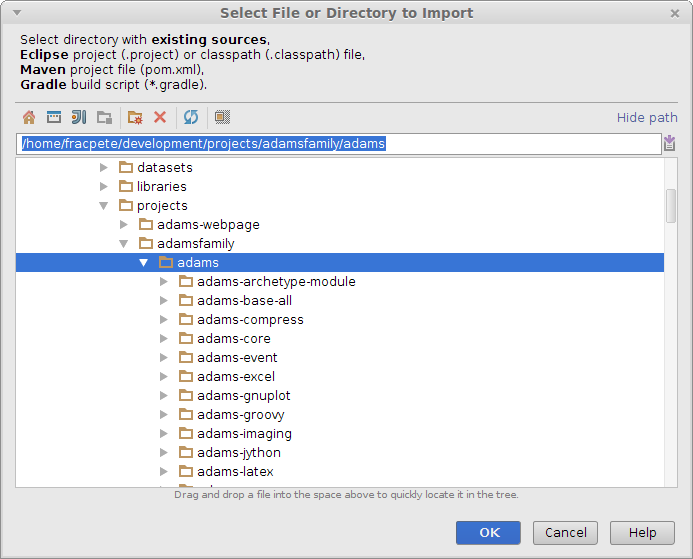
\includegraphics[width=10.0cm]{images/intellij-import_project-adams.png}
  \caption{IDEA: Selecting the project path.}
  \label{intellij-import_project-adams2}
\end{figure}
Then, select the top-level directory of ADAMS and import it as Maven project:
\begin{tight_itemize}
  \item import module from external model: Maven
  \item check \textit{import Maven projects automatically}
  \item check \textit{create module groups for multi-module Maven projects}
  \item select any relevant Maven profiles (or just use all of them)
\end{tight_itemize}
If you want to add other projects, like \textit{adams-addons} or
\textit{adams-incubator}, you must import them via
\textit{File -> Project structure...} from the main menu. There, select
\textit{Modules} and when clicking on the \textit{green plus sign}, select
\textit{Import module}.

Once you've imported ADAMS, you can configure the JDK that you want to use
(1.8 at the time of writing). For this, open \textit{Project structure} from
the main menu.

Under \textit{SDKs} you can define all the SDKs that you want to be able to use.
Simply click on the green plus and select the top-level directory of your JDK
(see Figure \ref{intellij-sdks}).
\begin{figure}[htb]
  \centering
  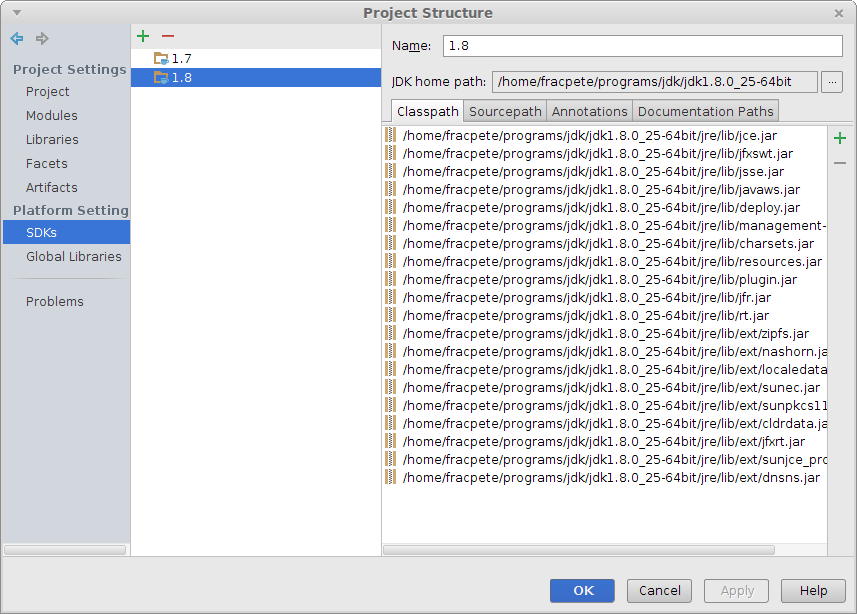
\includegraphics[width=10.0cm]{images/intellij-sdks.png}
  \caption{IDEA: Configuring the SDKs.}
  \label{intellij-sdks}
\end{figure}

And under \textit{Project}, you can then select the SDK that you want to use
for the current project (see Figure \ref{intellij-project-sdk}).
\begin{figure}[htb]
  \centering
  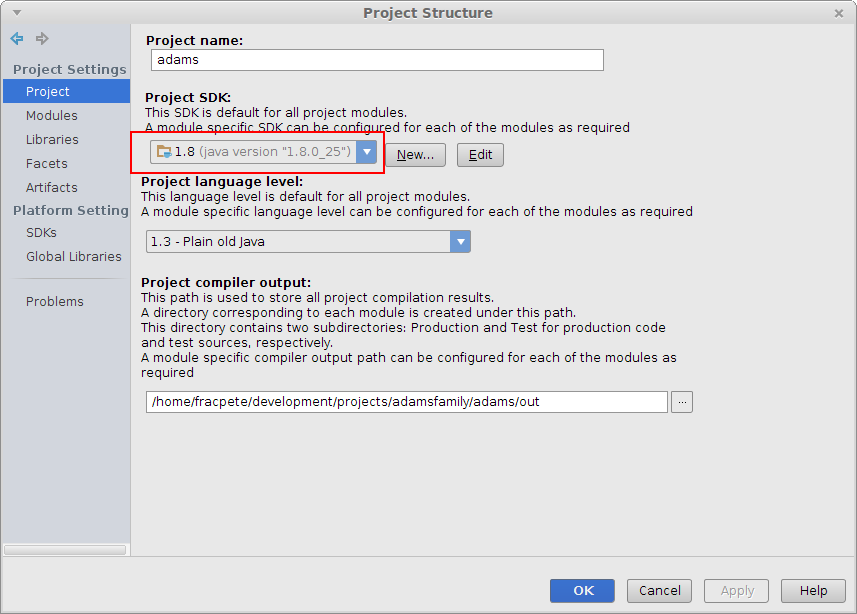
\includegraphics[width=10.0cm]{images/intellij-project-sdk.png}
  \caption{IDEA: Selecting the project SDK.}
  \label{intellij-project-sdk}
\end{figure}

ADAMS uses mixed spaces/tabs for indentation, with indentation being 2 spaces
and a tab representing 8 spaces. Figure \ref{intellij-indentation} shows where
to set these values.
\begin{figure}[htb]
  \centering
  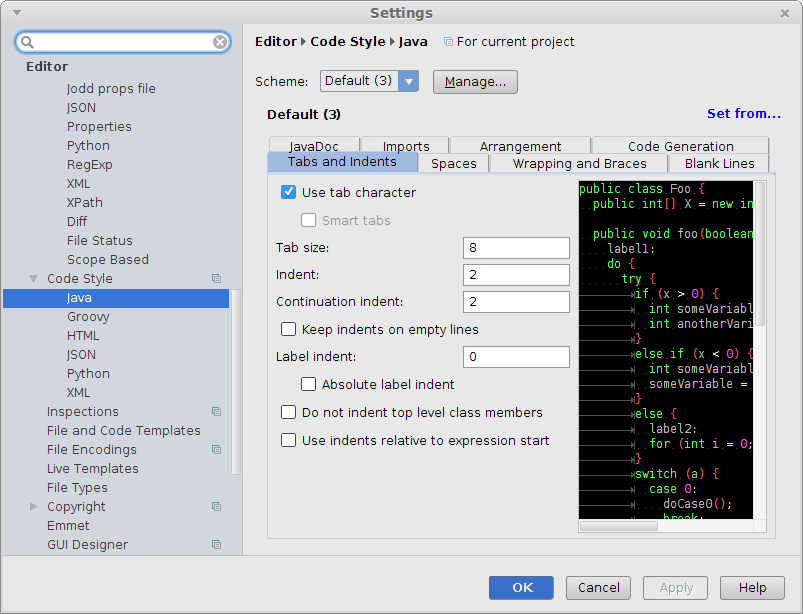
\includegraphics[width=10.0cm]{images/intellij-indentation.png}
  \caption{IDEA: Code formatting.}
  \label{intellij-indentation}
\end{figure}

Usually, you don't want to compile when you launch the application, but
whenever you change the code. Hence, enable "auto make", as shown in
Figure \ref{intellij-make}.
\begin{figure}[htb]
  \centering
  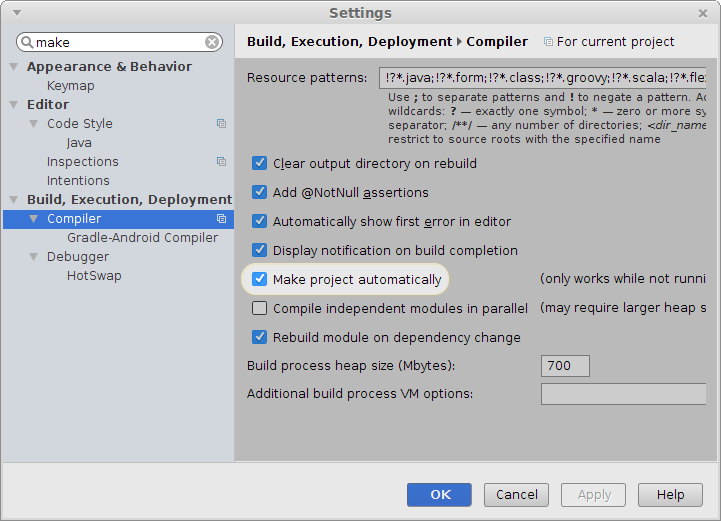
\includegraphics[width=10.0cm]{images/intellij-make.png}
  \caption{IDEA: Automatic compilation.}
  \label{intellij-make}
\end{figure}

Despite having \textit{auto make} enabled, it pays off to have a build
action before launching applications. Hence change the \textit{Before launch}
action to use \textit{Make, no error check}. Furthermore, you will most
likely have the module's top level directory as the default working directory
when starting up the application. You can set this using the
\texttt{$MODULE_DIR$} variable (see Figure \ref{intellij-app_defaults}).
\begin{figure}[htb]
  \centering
  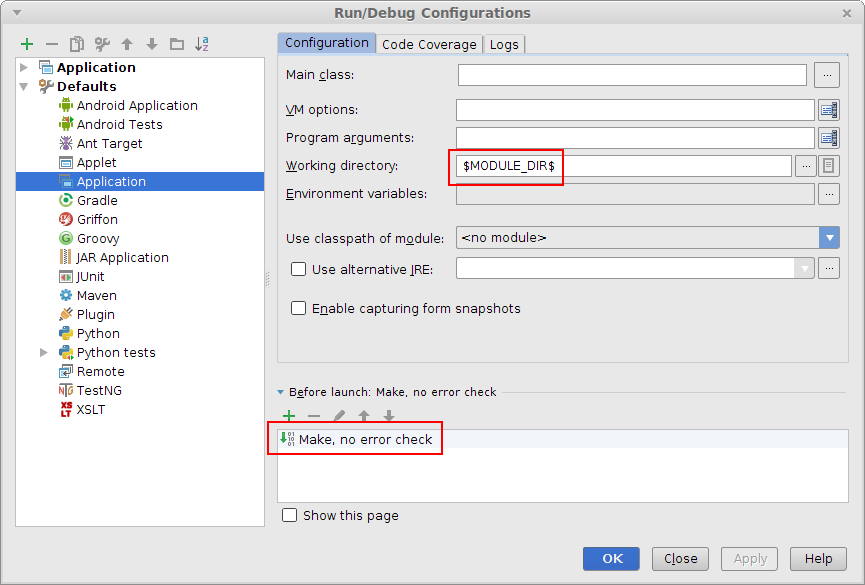
\includegraphics[width=10.0cm]{images/intellij-app_defaults.png}
  \caption{IDEA: Application defaults.}
  \label{intellij-app_defaults}
\end{figure}

For creating a launcher (or \textit{Run configuration}), you select
\textit{Run -> Edit configurations...} from the main menu. When clicking on
the green plus sign, use \textit{Application} as template and fill in
\texttt{adams.gui.Main} as the main class and the amount of RAM that you want
to use, eg 2GB (see Figure \ref{intellij-main}).
\begin{figure}[htb]
  \centering
  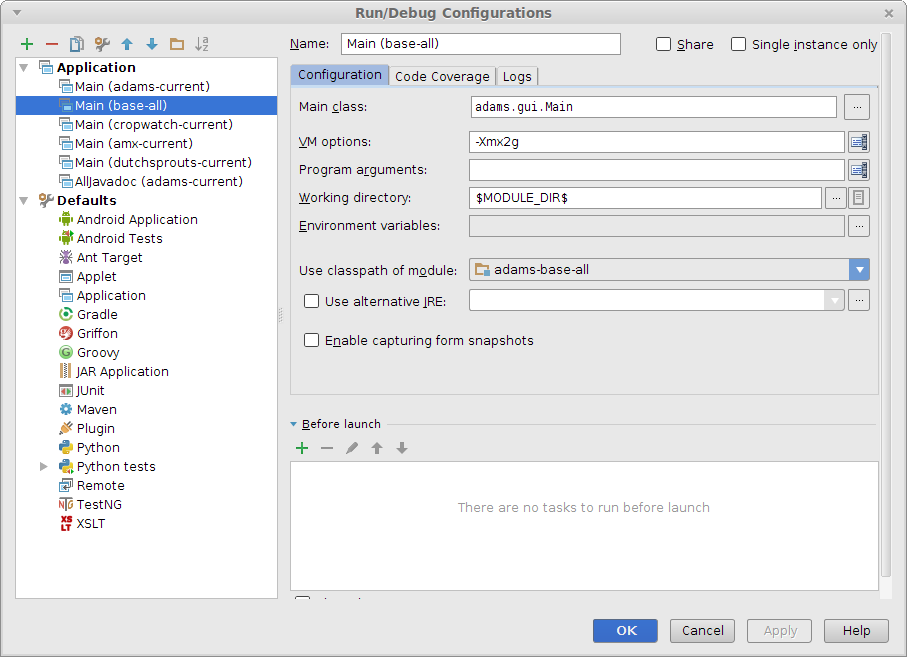
\includegraphics[width=10.0cm]{images/intellij-main.png}
  \caption{IDEA: Launching ADAMS.}
  \label{intellij-main}
\end{figure}

\clearpage
\section{Eclipse}
Prior to using IntelliJ IDEA, the choice of IDE was Eclipse\cite{eclipse}.
It offers great support for Maven and LaTeX - provided you install the proper
plug-ins.

\subsection{Plug-ins}
In order to get the most out of developing with Eclipse, it is recommended to
install the following plug-ins:
\begin{tight_itemize}
  \item m2e -- adds proper maven support \\
  \url{http://eclipse.org/m2e/}{}
  \item texlipse -- turns Eclipse into a type-setting environment with syntax
  highlighting, previewing, etc. This allows you to program and document with
  the same application. \\
  \url{http://texlipse.sourceforge.net/}{}
\end{tight_itemize}

Furthermore, install the \textit{buildhelper} m2e connector:
\begin{verbatim}
  Window
  -> Preferences
  -> Maven
  -> Discovery
\end{verbatim}

For viewing the source code correctly, use the following code formatting setup: \\
  \url{https://adams.cms.waikato.ac.nz/resources/eclipse-code-formatting.xml}{}

\subsection{Setting up ADAMS}
After installing the recommended plug-ins, you can proceed to import the ADAMS
source code that you checked out earlier using subversion.
Importing maven projects is extremely easy:
\begin{tight_itemize}
  \item right-click in the \textit{Navigator} or \textit{Project Explorer} and
  select \textit{Import...}
  \item select \textit{Maven} $\rightarrow$ \textit{Existing Maven projects}
  \item choose the top-level directory of your ADAMS source code tree (the one
  that contains all the modules and the system-wide \textit{pom.xml})
  \item select all the projects that you want to work with and hit
  \textit{Finish}
\end{tight_itemize}
For projects that have LaTeX documentation, you have to make sure that the
texlipse plugin is configured correctly, otherwise you might end up losing
files. Figure \ref{eclipse-texlipse_preferences} shows an example setup for the
manual of the \textit{adams-core} module. This module has the
\textit{adams-core-manual} sub-directory below the \textit{latex} directory,
with a LaTeX file of the same name, i.e., \textit{adams-core-manual.tex}. This
LaTeX file is listed as the main TeX file in the setup. Since the documentation
is generated using \textit{pdflatex}, the output format is \textit{pdf} and the
build command \textit{pdflatex}. It is very important not to place any temporary
files in the source directory, as they might get deleted during an Eclipse
\textit{clean project} operation. Instead, the output directory should be
\textit{target/latex/$<$documentation sub-dir$>$} (e.g.,
\textit{target/latex/adams-core-manual}), and the output file
\textit{target/latex/$<$documentation sub-dir$>$/$<$documentation
sub-dir$>$.pdf} (e.g., \textit{target/latex/adams-core-manual/adams-core-manual.pdf}).

\begin{figure}[htb]
  \centering
  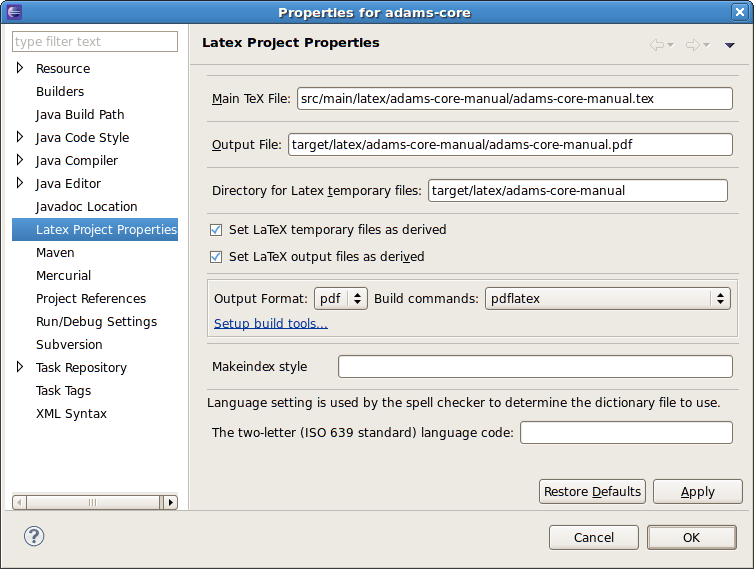
\includegraphics[width=10.0cm]{images/eclipse-texlipse_preferences.png}
  \caption{Eclipse: texlipse configuration for the \textit{adams-core} module.}
  \label{eclipse-texlipse_preferences}
\end{figure}

\section{Custom Maven project}
The ADAMS website allows you to create a custom Maven setup of a 
custom-tailored ADAMS distribution with just the modules that you want to 
include. You can access this functionality here: \\
  \url{https://adams.cms.waikato.ac.nz/roll-your-own}{} \\
Figure \ref{rollyourown} shows a screenshot of the website.

\begin{figure}[htb]
  \centering
  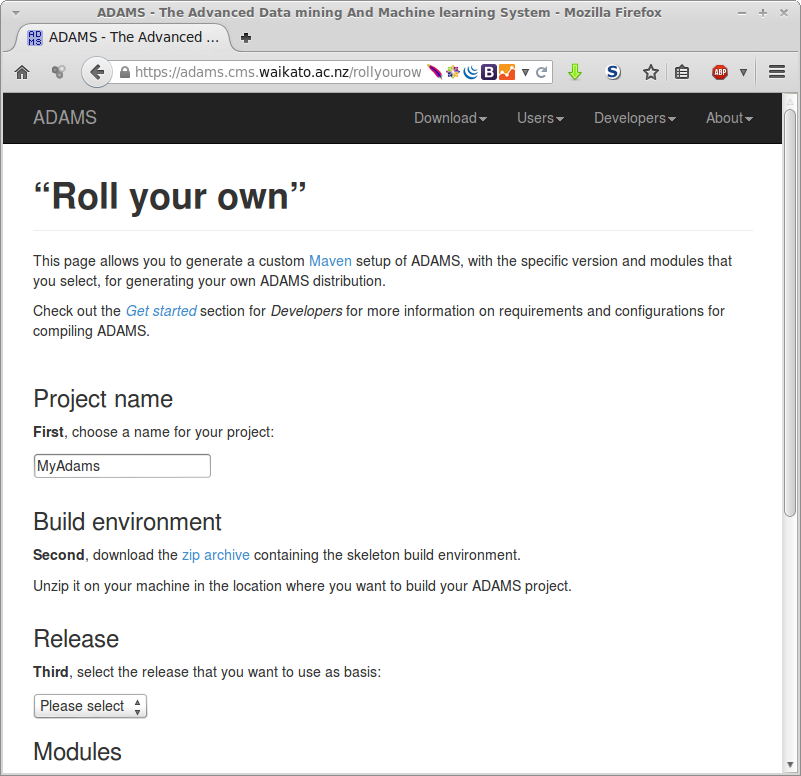
\includegraphics[width=10.0cm]{images/rollyourown.png}
  \caption{Screenshot of the ``Roll your own'' section of the ADAMS website.}
  \label{rollyourown}
\end{figure}

\section{Non-maven approach}
Though it is recommended, the use of Maven is not required. If you download
a release or snapshot of ADAMS, you can simply link your project against all
the jars in the \texttt{lib} directory for compiling your code.

Creating a new release can be done like this as well: simply drop any 
additional jars that your project requires and/or generates in the \texttt{lib}
directory. You only need to create a new archive from the ADAMS directory to
get an extended ADAMS release/snapshot. No need to update any scripts, as all
jars in the \texttt{lib} directory get added to the classpath automatically.

When using Eclipse or IntelliJ IDEA with this approach, the only disadvantage is that you will
have to manually attach the sources to the project (located in the 
\texttt{src} directory). Otherwise you won't be able to view ADAMS classes
as source code. This is something that gets handled automatically by the
\textit{m2e} Eclipse plugin for Maven.

%%%%%%%%%%%%%%%%%
% Using the API %
%%%%%%%%%%%%%%%%%
\chapter{Using the API}
Using the graphical user interface may be sufficient for most users, but as soon
as you want to embed one framework in another, you need to get down and dirty
with the API. This chapter addresses some core elements of the ADAMS API, mainly
the flow related APIs.

\section{Flow}
The API of the flow component of ADAMS is simple by design. The idea was to
provide not just a graphical interface for setting up and manipulating flows,
but also enabling other people for embedding flows in their own code. Limiting
the interface to only a few methods was therefore necessary. The following 
sections provide an in-depth discussion of the API.

\subsection{Life-cycle of an actor}
Any actor, whether a simple one like the \textit{Display} actor or a control
actor like \textit{Branch}, has the following lifecycle of method calls:
\begin{tight_itemize}
  \item \textbf{setUp()} -- performs initializations and checks, ensuring that
  the actor can be executed
  \item \textbf{execute()} -- executes the actor, i.e., transformers process the
  input data and generate output data
  \item \textbf{wrapUp()} -- finishes the execution, frees up some memory that
  was allocated during execution
  \item \textbf{cleanUp()} -- removal of graphical output, like dialogs/frame
  and destruction of internal data structures
\end{tight_itemize}
The \textit{setUp()} and \textit{execute()} methods return
\textit{null} if everything was OK, otherwise the reason (i.e., error message) why
the method didn't succeed. The \textit{execute()} method is executed as long as
\textit{finished()} returns \textit{false}.

\heading{OutputProducer}
As long as the \textit{hasPendingOutput()} method of an actor implementing
\textit{OutputProducer} returns \textit{true}, output tokens will get collected
and passed on to the next \textit{InputConsumer}.

\subsection{Setting up a flow}
ADAMS distinguishes between primitive actors, like the \textit{Display} actor,
and ones that handle other actors, like the \textit{Branch} actor. The 
\textit{actor handlers} can be divided into ones that have a fixed number
of sub-actors, like the \textit{IfThenElse} actors (always two sub-actors),
and others that can have a more or less arbitrary number of sub-actors (a 
lower bound may be defined, though), like the \textit{Branch} actor.

Usually, the \textit{Flow} control actor is the outermost actor. But this is
not necessary. In theory, any actor can be setup, executed and destroyed again.
Only if you need things like variables and internal storage, you will need a 
control actor like the \textit{Flow} actor to provide this kind of functionality.

Setting up a flow conists basically of nesting the actors like in the flow
editor. The tree structure in the flow editor is a 1-to-1 representation of the
underlying actor nesting. For actors that handle sub-actors (implementing the
\textit{ActorHandler} interface), you can use the \texttt{set(int,
AbstractActor)} method for setting/replacing a sub-actor at the specified index.
Actors that implement the \textit{MutableActorHandler} interface instead, adding
of new actors is much simpler: either using the \texttt{add(AbstractActor)}
method (appends the actor at the end) or \texttt{add(int, AbstractActor)}, which
adds/inserts the actor at the specified location. To remove any previous 
existing actors, you can call the \texttt{removeAll()} method. Instead of adding
the actors one-by-one, some actors (mainly \textit{MutableActorHandler} ones) 
offer methods for setting/getting an array of sub-actors, like the 
\texttt{setActors} and \texttt{getActors} methods of the \textit{Flow} actor.

The following piece of code sets up a little flow that generates a number
of random numbers between 100 and 200, which get used as input in a mathematical 
expression (simply dividing the numbers by PI), before dumped them into a 
text file in the temp directory.
\begin{verbatim}
import adams.flow.control.Flow;
import adams.flow.source.RandomNumberGenerator;
import adams.data.random.JavaRandomInt;
import adams.flow.transformer.MathExpression;
import adams.parser.MathematicalExpressionText;
import adams.flow.sink.DumpFile;
import adams.core.io.PlaceholderFile;
...
Flow flow = new Flow();

RandomNumberGenerator rng = new RandomNumberGenerator();
rng.setMaxNum(10);
JavaRandomInt jri = new JavaRandomInt();
jri.setMinValue(100);
jri.setMaxValue(200);
rng.setGenerator(jri);
flow.add(rng);

MathExpression math = new MathExpression();
MathematicalExpressionText expr = new MathematicalExpressionText();
expr.setValue("X / PI");
math.setExpression(expr);
flow.add(math);

DumpFile df = new DumpFile();
df.setOutputFile(new PlaceholderFile("${TMP}/random.txt"));
flow.add(df);
\end{verbatim}

%%%%%%%%%%%%%%%%%%%
% Extending ADAMS %
%%%%%%%%%%%%%%%%%%%
\chapter{Extending ADAMS}
The overarching goal of ADAMS was to develop a plug-in framework, which makes
extending it very easy. The built-in dynamic class discovery is at the heart of
it. The following sections cover various aspects of extending ADAMS, from merely
adding a subclass to creating a new project built on top of ADAMS.

\section{Dynamic class discovery}
\label{dynamic_class_discovery}
ADAMS is a flexible plug-in framework thanks to the dynamic class discovery that
is offered through the \texttt{adams.core.ClassLocator} class. But merely
locating classes is just half of the story, you also have to organize them. This
is where the \texttt{adams.core.ClassLister} class and its properties file
\texttt{ClassLister.props} (located in the \texttt{adams.core} package, below
\texttt{src/main/resources}) come into play. The \texttt{ClassLister} class
iterates through the keys in the properties file, which are names of
superclasses, and locates all the derived classes in the listed packages, the
comma-separated list which represents the value of the property.

Here is an example for the conversion schemes that can be used with the
\textit{Convert} transformer:
\begin{verbatim}
  adams.data.conversion.AbstractConversion=\
    adams.data.conversion
\end{verbatim}
The superclass in this case is
\texttt{adams.data.conversion.AbstractConversion} and only one package is listed
for exploration, \texttt{adams.data.conversion}.

Instead of adding new keys and packages to this central properties file,
whenever a new modules requires additional class discovery, the developer can
just simply add an extra file in their module. The only restriction is that it
has to be located in the \texttt{adams.core} package (below
\texttt{src/main/resources}).

This works for adding new keys, i.e., new superclasses, as well as for merely
adding additional packages to existing superclasses. In the latter case, only
the additional packages have to be specified, since ADAMS will automatically
merge keys across multiple properties files.

\subsection{Additional package}
Coming back to the previous example of the conversion schemes, module
\textit{funky-module}, package \texttt{org.funky.conversion} contains
additional conversion schemes. These are all derived from
\texttt{AbstractConversion}. In that case, the \texttt{ClassLister.props} file
would contain the following entry:
\begin{verbatim}
  adams.data.conversion.AbstractConversion=\
    org.funky.conversion
\end{verbatim}
When starting up, ADAMS will merge the two props files and the key
will look like this, listing both packages:
\begin{verbatim}
  adams.data.conversion.AbstractConversion=\
    adams.data.conversion,\
    org.funky.conversion
\end{verbatim}

\subsection{Additional class hierarchy}
Adding a new class hierarchy works just the same. You merely have to use the
superclass that all other classes are derived from as key in the props file and
list all the packages to look for derived classes. Here is an example for a
class hierarchy derived from \texttt{org.funky.AbstractFunkiness}, which has
derived classes in the packages \texttt{org.funky} and \texttt{org.notsofunky}:
\begin{verbatim}
  org.funky.AbstractFunkiness=\
    org.funky,\
    org.notsofunky
\end{verbatim}

\subsection{Blacklisting classes}
In production environments it might not always be wise to list all the classes
that are available, e.g., experimental classes. ADAMS provides a mechanism to
exclude certain classes, using pattern matching (using regular expressions).
These patterns are listed in the \texttt{ClassLister.blacklist} properties file.
The format for this file is similar to the \texttt{ClassLister.props} file, with
the \textit{key} being the superclass and the \textit{value} a comma-separated
list of patterns. In the following an example that excludes a specified data
conversion class called \texttt{SuperExperimentalConversion} from being listed:
\begin{verbatim}
  adams.data.conversion.AbstractConversion=\
    org\.funky\.conversion\.SuperExperimentalConversion
\end{verbatim}
If you want to exclude all conversions of the \texttt{og.funk.conversion}
package that contain the word \textit{Experimental}, then use the following
pattern:
\begin{verbatim}
  adams.data.conversion.AbstractConversion=\
    org\.funky\.conversion\..*Experimental.*
\end{verbatim}

\section{Creating a new actor}
Being a workflow-centric application, it is most likely the case that a new
module will contain new actors and not just newly derived subclasses of already
existing superclasses. For this reason, the development of new actors is
explained in detail.

Developing a new actor is fairly easy, you only need to do the following:
\begin{tight_itemize}
	\item create a new class
	\item create an icon, which is displayed in the flow editor
	\item \textit{[optional, but recommended]} create a JUnit test for the actor
\end{tight_itemize}

\subsection{Creating a new class}
Any actor has to be derived from \textit{adams.flow.core.AbstractActor}.
Depending on whether the actor consumes or produces data, there are two more
interfaces available:
\begin{tight_itemize}
	\item \textit{adams.flow.core.InputConsumer} -- for actors that process data
	that they receive at their input
	\item \textit{adams.flow.core.OutputProducer} -- for actors that generate data
	of some form
\end{tight_itemize}

In general, four types of actors can be distinguished, based on the combinations
of these two interfaces:
\begin{tight_itemize}
	\item \textit{standalone} -- no input, no output
	\item \textit{source} -- only output
	\item \textit{transformer} -- input and output
	\item \textit{sink} -- only input
\end{tight_itemize}
In order to make development of new actors easier and to avoid duplicate code
as much as possible, there are already a bunch of abstract classes in ADAMS
that implement these interfaces:
\begin{tight_itemize}
	\item \textit{adams.flow.standalone.AbstractStandalone} -- for standalones
	\item \textit{adams.flow.source.AbstractSource} -- for data producing source actors
	\item \textit{adams.flow.transformer.AbstractTransformer} -- for simple transformers
    that take one input token and generate at most one output token.
	\item \textit{adams.flow.sink.AbstractSink} -- the ancestor of all sinks, actors that
    only consume data
\end{tight_itemize}
There are plenty more abstract super classes, since there are actors that
perform similar tasks. Some of them are listed below:
\begin{tight_itemize}
	\item \textit{adams.flow.sink.AbstractDisplay} -- for actors displaying data in a
    frame or dialog
	\item \textit{adams.flow.sink.AbstractGraphicalDisplay} -- for actors that display
    graphical data, e.g., a graph, which can be saved to an image file automatically
	\item \textit{adams.flow.sink.AbstractTextualDisplay} -- for actors that display text
\end{tight_itemize}
A special interface, \textit{adams.flow.core.ControlActor}, is an indicator
interface for actors that control the flow or the flow of data somehow. For
instance, a \textit{Branch} actor controls the flow of data, since it provides
each sub-branch with the same data token that it received.

Actors that manage sub-actors, need to implement the
\textit{adams.flow.core.ActorHandler} interface.

The special superclass \textit{adams.flow.control.AbstractControlActor} already
implements the \textit{ActorHandler} and \textit{ControlActor} interfaces and
implements some of the functionality. The \textit{AbstractConnectorControlActor}
class in the same package, is used for control actors which sub-actors are
connected, like the \textit{Sequence} actor. The sub-actors in the
\textit{Branch} actor, on the other hand, are not connected, but treated
individually.

The following methods you will usually have to implement:
\begin{tight_itemize}
	\item \texttt{globalInfo()} -- The general help text for the actor.
	\item \texttt{doExecute()} -- Here the actual execution code is located, the
	\texttt{pre}- and \texttt{post}- methods, you usually won't have to touch. All
	three methods are called in the \texttt{execute()} method.
\end{tight_itemize}

\subsection{Option handling}
Option handling in ADAMS is available through classes implementing the
\texttt{OptionHandler} interface (package \texttt{adams.core.option}). Most
classes or class hierarchies, that includes the actors, are simply
derived from \texttt{AbstractOptionHandler}, which implements this
interface and all the required methods. For adding a new option, there
are usually only three things to do:
\begin{tight_enumerate}
	\item add the (protected) \textbf{field}
	\item add the \texttt{get}-, \texttt{set}- and
	\texttt{tiptext}-\textbf{methods} that make up the new property of this class
	\item add an option \textbf{definition}
\end{tight_enumerate}

\subsubsection{Example}
The following shows how to implement a new option for an integer field
\textit{volume} that only allows values from 1 to 11. For clarity's sake,
Javadoc comments have been left out. 

\noindent First of all, we define the (serializable) field:
{\small
\begin{verbatim}
  protected int m_Volume;
\end{verbatim}
}

\noindent Then we add the required methods\footnote{The tiptext method generates
the help text in the GUI and command-line, so you should never omit this.}:
{\small
\begin{verbatim}
  public void setVolume(int value) {
    if (getOptionManager().isValid("volume", value))  // checks numeric bounds
      m_Volume = value;
      reset();   // notify object that the settings have changed
    }
  }
  public int getVolume() {
    return m_Volume;
  }
  public String volumeTipText() {
    return "The volume to crank up the speakers to.";
  }
\end{verbatim}
}

\noindent And finally, we define the option, by overriding the
\texttt{defineOptions()} method. Otherwise, the option won't show up in the GUI and you won't be able to
set the value via a command-line string.
{\small
\begin{verbatim}
  public void defineOptions() {
    super.defineOptions();
    m_OptionManager.add(
	    "volume",    // flag on the command-line without the leading "-"
	    "volume",    // the Java Bean property for getting/setting the value
	    1,           // the default volume
	    1,           // the minimum value
	    11);         // the maximum value
  }
\end{verbatim}
}
For numeric values, like integers and doubles, you can specify the lower and
upper bounds, if that makes sense, like in our example here. If one of them is
to be unbounded, simply use \texttt{null}. If both are unbounded, then simply
omit the last two parameters.

\subsection{Variable side-effects}
Actors keep track of variables that have been attached to either one of their
own options (e.g., \textit{fieldIndex} option of the \textit{StringCut} 
transformer) or to options of one their sub-objects (e.g., the 
\textit{numDecimals} option of the \textit{DoubleToString} conversion used
by the \textit{Convert} transformer). Options like sub-actors, as used by 
actor handlers such as \textit{Tee} or \textit{Branch}, are excluded from this
monitoring.

Attaching a variable to an option has some side-effects that you need to be 
aware of when variable values change:
\begin{tight_itemize}
	\item affected actors get re-initialized, since the configuration has 
	changed, resuling in calls of the \textit{reset()} and \textit{setUp()} 
	methods.
	\item actor handlers recursively call the \textit{setUp()} of their 
	sub-actors.
\end{tight_itemize}
In order to prevent losing the internal state, due calling the \textit{reset()}
method, you can backup the current state of member variables in an actor. For
instance, the \textit{Count} control actor keeps track how many tokens have 
passed through. This counter gets zeroed when calling \textit{reset()}. You can 
backup/restore the current state using the \textit{backupState} and 
\textit{restoreState} methods. These methods use an internal hashtable to backup
key-value pairs. The following code is used by \textit{Count} to backup the 
counter \textit{m\_Current}:
{\small
\begin{verbatim}
  public final static String BACKUP_CURRENT = "current";

  protected Hashtable<String,Object> backupState() {
    Hashtable<String,Object> result = super.backupState();
    result.put(BACKUP_CURRENT, m_Current);
    return result;
  }

  protected void restoreState(Hashtable<String,Object> state) {
    if (state.containsKey(BACKUP_CURRENT)) {
      m_Current = (Integer) state.get(BACKUP_CURRENT);
      state.remove(BACKUP_CURRENT);
    }
    super.restoreState(state);
  }
\end{verbatim}
}
Of course, this counter now never gets zeroed, since we back it up all the time.
In order to zero the internal counter, i.e., if an option of the \textit{Count} 
actor itself was modified and it should get zeroed, you have to \textit{prune}
the backup. You can do this by using the \textit{pruneBackup} method, which gets 
called in case one of its own members got modified. The code to achieve this is 
as follows:
{\small
\begin{verbatim}
  protected void pruneBackup() {
    super.pruneBackup();
    pruneBackup(BACKUP_CURRENT);
  }
\end{verbatim}
}

\subsection{Graphical output}
Using the \texttt{AbstractGraphicalDisplay} as superclass instead of
\texttt{AbstractDisplay}, allows you to take advantage of some additional
functionality: menu, \textit{SendTo} framework integration.

Methods that require implementation are as follows:
\begin{tight_itemize}
	\item \texttt{globalInfo()} -- a short description of the sink, available 
	as help in the GUI
	\item \texttt{accepts()} -- the classes that this sink can process and 
	display
	\item \texttt{newPanel()} -- generates the panel that is added to the 
	dialog
	\item \texttt{clearPanel()} -- removes the currently displayed data
	\item \texttt{display(Token)} -- processes and displays the content of
	the token provided (of one of the accepted classes)
\end{tight_itemize}
If it is necessary to extend the default menu, you can override the 
\texttt{createMenuBar()} method, which generates the \texttt{JMenuBar} that
is used in the dialog.

It is recommended to implement the \texttt{DisplayPanelProvider} interface as
well. By doing this, the sink can be selected in the \texttt{DisplayPanelManager}
sink, which keeps a \textit{graphical} history of the tokens passing through,
by creating a single panel per token.

\subsection{Textual output}
Instead of directly sub-classing \texttt{AbstractDisplay}, you should use
\texttt{AbstractTextualDisplay} instead. This abstract class already implements
various interfaces like \texttt{MenuBarProvider} and
\texttt{SendToActionSupporter}, to provide the user with a menu for saving the 
output, changing font size, etc and also enabling the user to take advantage 
of the \textit{SendTo} framework. In the simplest case, this is printing the
textual output on a printer.

You only need to implement the following methods in order to get a fully 
functional interface:
\begin{tight_itemize}
	\item \texttt{globalInfo()} -- a short description of the sink, available 
	as help in the GUI
	\item \texttt{accepts()} -- the classes that this sink can process and 
	display
	\item \texttt{newPanel()} -- generates the panel that is added to the 
	dialog
	\item \texttt{clearPanel()} -- clears the (textual) content of the panel
	\item \texttt{display(Token)} -- processes and displays the content of
	the token provided (of one of the accepted classes)
	\item \texttt{supplyText()} -- returns text that is currently on display
\end{tight_itemize}
If it is necessary to extend the default menu, you can override the 
\texttt{createMenuBar()} method, which generates the \texttt{JMenuBar} that
is used in the dialog.

\subsection{Creating an icon}
The icon has to be placed in the \textit{adams.gui.images} package with the same
name as the class, but with a GIF or PNG extension. E.g., the \textit{Display}
actor's full class name is \textit{adams.flow.sink.Display}. This means that
ADAMS expects an image \textit{called adams.flow.sink.Display.gif} or
\textit{adams.flow.sink.Display.png} in the \textit{adams.gui.images} package.
NB: Since ADAMS uses Maven as build system, non-Java files need to placed below
the \textit{src/main/resources} directory.

There are already some templates available for new icons:
\begin{tight_itemize}
	\item \textit{adams.flow.standalone.Unknown.gif} -- red outline
	\item \textit{adams.flow.source.Unknown.gif} -- orange outline
	\item \textit{adams.flow.transformer.Unknown.gif} -- green outline
	\item \textit{adams.flow.sink.Unknown.gif} -- grey outline
	\item \textit{adams.flow.control.Unknown.gif} -- blue outline
\end{tight_itemize}
Just create a copy of one of these icons and modify it to make your actor
distinguishable from all the others in the flow editor.

\subsection{Creating a JUnit test}
JUnit 3.8.x  \cite{junit} is used as basis for the unit tests. Test classes are
placed in \textit{src/test/java} and have to be suffixed with \textit{Test}.
E.g., the \textit{Display} actor has a test class called \textit{DisplayTest}
in package \textit{adams.flow.sink}.

A flow unit test needs to be derived from \textit{adams.flow.AbstractFlowTest}
and only the \textit{getActor()} method needs to be implemented by default. This
method typically returns a Flow actor which is set up and executed. If any step
in the lifecycle of the actor returns an error, the unit test will fail.

If required, a regression test can be performed. For this, you merely need to
implement a method called \textit{testRegression()}, which calls the
\textit{performRegressionTest(File)} or \textit{performRegressionTest(File[])}
method. These methods record the content of the specified files in a special
reference file (found below \textit{src/test/resources}) and the next
time the test is run the newly generated output is compared against the stored
reference data. If the data differs, the regression test will fail. Please note,
that you should remove temporary files that you use for regression tests in the
\textit{setUp()} and \textit{tearDown()} methods of the unit test, to provide a
clean environment to this and other tests.

\section{Creating a new module}
First, you have to make sure that your local repository catalog is up-to-date:
\begin{verbatim}
mvn archetype:update-local-catalog
\end{verbatim}
Second, run the following command to create a new module called
\textit{adams-funky}:
\begin{verbatim}
mvn archetype:generate \
     -DarchetypeCatalog=local \
     -DinteractiveMode=false \
     -DarchetypeGroupId=nz.ac.waikato.cms.adams \
     -DarchetypeArtifactId=adams-archetype-module \
     -DarchetypeVersion=0.4.10 \
     -DgroupId=nz.ac.waikato.cms.adams \
     -DartifactId=adams-funky \
     -Dversion=0.0.1-SNAPSHOT
\end{verbatim}
This command will base the module on the latest ADAMS release,
using the \texttt{0.4.10} release of the template (or \textit{archetype}, to use
the correct maven term). The version number of the newly created module will be
\texttt{0.0.1-SNAPSHOT}.

After the command has finished, you have to update the \textit{Module.props}
file in the \textit{src/main/resources1/adams/env} directory. The minimal change
that you have to perform is to set the correct module name, specified under the
\textit{Name} key. Apart from the name, this properties file contains
information about your module, which gets displayed automatically in the
\textit{About} dialog in the GUI.

\heading{Official modules}
If you run the above command within the top-level directory that hosts all the
other ADAMS modules, then it will automatically add this module to the
\texttt{pom.xml} configuration file as a new dependent module. This means that
each time you issue a command in this directory (e.g., \texttt{mvn package}),
your module will be processed accordingly. This is the preferred approach when
adding a new module to be added to the ADAMS subversion repository.

\heading{Other modules}
Otherwise, if you created that module outside the ADAMS module hierarchy, it
will use the artifacts that you have installed in your local repository (of
course, maven will occasionally check the Nexus repository manager for updates).
Use this approach if there is no intention on adding the module to the official
ADAMS subversion repository.

\section{Main menu}
\label{mainmenu}
The main menu of ADAMS can use a pre-defined menu structure, as defined in the
\texttt{adams/gui/Main.props} properties file. But it also offers dynamic
addition of other menu items at runtime.

In order for new menu items being picked up at runtime, you need to derive a
new menu item definition from the following class (or one of the appropriate
abstract classes derived from it):
\begin{verbatim}
  adams.gui.application.AbstractMenuItemDefinition
\end{verbatim}
For instance, if you merely want the menu item to open a browser with a specific
URL (displaying the homepage or some help page), then you can derive the menu
item from the following class:
\begin{verbatim}
  adams.gui.application.AbstractURLMenuItemDefinition
\end{verbatim}
If you don't want to modify the dynamic class discovery
(\texttt{ClassLister.props}), then you have to place your newly created menu
item definition in the following package:
\begin{verbatim}
 adams.gui.menu
\end{verbatim}
In order to get implement a menu item, derived from
\texttt{AbstractMenuItemDefinition}, you need to implement or override the
following methods:
\begin{tight_itemize}
	\item \textit{getTitle()} -- The text of the menu item.
	\item \textit{getIconName()} -- By default, the menu item won't have an icon,
	specify the filename (without path) of the icon that you would like to use. The
	icon is expected to reside in the \textit{adams/gui/images} directory.
	\item \textit{getCategory()} -- This string defines the menu the item will get
	added to. Existing ones are, e.g., \textit{Tools} or \textit{Maintenance}. You
	don't have to use an existing one, new categories get automatically added as
	new menus.
	\item \textit{isSingleton()} -- If your menu item can be launched multiple
	times, then return \textit{false}, otherwise \textit{true}.
	\item \textit{getUserMode()} -- This defines the visibility of your menu item.
	Whether it is intended for regular users, experts or developers. What level is
	being displayed is defined -- normally -- by the application's
	\textit{--user-mode $<$mode$>$} command-line option when starting the
	application.
	\item \textit{launch()} -- This method finally launches your custom code. More
	details below.
\end{tight_itemize}

\heading{The \textit{launch()} method}
For the best integration within ADAMS, the \textit{launch()} will create a
\textit{java.swingx.JPanel} derived panel and create an internal frame using the
following call:
\begin{verbatim}
  JPanel panel = new MyFunkyPanel();
  ChildFrame frame = createChildFrame(panel);
\end{verbatim}
Using this approach, your panel with show up in the \textit{Windows} menu of the
main menu of ADAMS.

Menu items derived from \textit{AbstractURLMenuItemDefinition} don't need to
implement this method, they merely need to supply a URL string with the
\textit{getURL()} method. Their \textit{launch()} method uses this URL to open a
browser with.

\section{Flow editor}
The flow editor itself allows for some customization:
\begin{tight_itemize}
  \item Adding menu items to the main menu.
  \item Changing the layout of the tree popup menu.
\end{tight_itemize}

\subsection{Main menu}
\label{floweditor_mainmenu}
The flow editor can add new menu items dynamically to its main menu. You can
only need to derive a new class from the following abstract superclass and
place it in the \texttt{adams.gui.flow.menu} package (or update the
\texttt{ClassLister.props} file accordingly if in another package):
\begin{verbatim}
  adams.gui.flow.menu.AbstractFlowEditorMenuItem
\end{verbatim}
When you implement your new class, you need to do three things:
\begin{tight_enumerate}
  \item Determine in which menu the item should get added (you can start a new
  menu as well).
  \item Create the \texttt{AbstractBaseAction} that does the actual work and
  also defines how your menu item looks.
  \item React to updates in the user interface.
\end{tight_enumerate}
Here is an example class, called \texttt{RunningHelloWorld}, which is available
if there is at least one flow currently running. The menu item titled ``Say hi'' 
simply pops up a dialog with the words ``Hello World!''.
{\scriptsize
\begin{verbatim}
package adams.gui.flow.menu;
  
import adams.gui.action.AbstractBaseAction;
import adams.gui.core.GUIHelper;
import adams.gui.flow.FlowEditorPanel;

public class RunningHelloWorld extends AbstractFlowEditorMenuItem {
  // we want to add our menu item to the "View" menu
  public String getMenu() {
    return FlowEditorPanel.MENU_VIEW;
  }
  // the action that handles the dialog
  protected AbstractBaseAction newAction() {
    return new AbstractBaseAction("Say hi") {
      GUIHelper.showInformationMessage(getOwner(), "Hello World!");
    }
  }
  // action is only available if at least one flow is running
  public void updateAction() {
    m_Action.setEnabled(getOwner().isAnyRunning());
  }
}
\end{verbatim}
}
Shortcuts definitions can be stored in the \texttt{FlowEditorShortcuts.props}
files (package \texttt{adams.gui.flow}, below \texttt{src/main/resources}). The
definition can be accessed and converted into a \texttt{KeyStroke} object using
the the following call:
\begin{verbatim}
  adams.gui.core.GUIHelper.getKeyStroke(
      adams.gui.flow.FlowEditorPanel.getEditorShortcut("File.New"));
\end{verbatim}
This example accesses the shortcut definition stored in property
\texttt{Shortcuts.File.New}.

\subsection{Popup menu}
\label{floweditor_popupmenu}
Each item in the popup menu that is displayed in the tree when opening the
right-click menu for one or more actors is derived from the following class:
\begin{verbatim}
  adams.gui.flow.tree.menu.AbstractTreePopupMenuItem
\end{verbatim}
Even sub-menus are derived from this superclass, but instead of returning a
simple \texttt{JMenuItem} object in the \texttt{getMenuItem(StateContainer)}
method, a \texttt{JMenu} object is returned, which encapsulates other menu
items.

The layout of this popup menu is defined in the \texttt{FlowEditor.props} file,
in the \texttt{adams.gui.flow} package (below the \texttt{src/main/resources}
directory). The key for the menu is called \texttt{Tree.PopupMenu} and the value
for this property is a simple comma-separated list of class names (use ``-''
if you want to add a separator).

Shortcuts definitions can be stored in the \texttt{FlowEditorShortcuts.props}
files (package \texttt{adams.gui.flow}, below \texttt{src/main/resources}). The
definition can be accessed and converted into a \texttt{KeyStroke} object using
the the following call:
\begin{verbatim}
  adams.gui.core.GUIHelper.getKeyStroke(
      adams.gui.flow.FlowEditorPanel.getTreeShortcut("Help"));
\end{verbatim}
This example accesses the shortcut definition stored in property
\texttt{Tree.Shortcuts.Help}.

The following example menu item pops up a ``Hello World!'' dialog if the
flow/actor is editable:
{\scriptsize
\begin{verbatim}
package adams.gui.flow.tree.menu;

import java.awt.event.ActionEvent;
import java.awt.event.ActionListener;
import javax.swing.JMenuItem;
import adams.gui.core.GUIHelper;
import adams.gui.flow.tree.StateContainer;

public class HelloWorldItem extends AbstractTreePopupMenuItem {
  protected JMenuItem getMenuItem(final StateContainer state) {
    JMenuItem result = new JMenuItem("Hello world");
    result.setEnabled(getShortcut().stateApplies(state));
    result.setAccelerator(getShortcut().getKeyStroke());
    result.addActionListener(new ActionListener() {
      public void actionPerformed(ActionEvent e) {
        getShortcut().execute(state);
      }
    });
    return result;
  }
  protected AbstractTreeShortcut newShortcut() {
    return new AbstractTreeShortcut() {
      protected String getTreeShortCutKey() {
 	   return "HelloWorld";   // won't do anything unless props file is updated
      }
      public boolean stateApplies(StateContainer state) {
        return state.editable;
      }
      protected void doExecute(StateContainer state) {
        GUIHelper.showInformationMessage(state.tree, "Hello World!");
      }
    };
  }
}
\end{verbatim}
}

\section{Image viewer}
The Image viewer allows you to add custom plugins to the menu. The superclass
for all plugins is:
\begin{verbatim}
  adams.gui.visualization.image.plugins.AbstractImageViewerPlugin
\end{verbatim}
\begin{tight_itemize}
  \item \textit{canExecute(ImagePanel)} -- determines whether the plugin can
  be applied to the current image panel.
  \item \textit{doExecute()} -- executes the plugin and returns a string
  depending on success (\textit{null}) or failure (\textit{error message}).
  \item \textit{createLogEntry()} -- can be used to output a string that 
  should appear the in viewer's log tab; return \textit{null} if that does
  not apply.
\end{tight_itemize}

\section{Database access}
In order to add support in ADAMS for a database, in addition to MySQL\footnote{\url{http://www.mysql.com/}{}} 
and sqlite\footnote{\url{http://www.sqlite.org/}{}}, the following steps
are required:
\begin{itemize}
	\item Add a dependency for the JDBC driver to your \textit{pom.xml} project
	definition (search on Maven Central\footnote{\url{http://search.maven.org/}{}}). 
	For instance, adding the Oracle JDBC driver: \\
\begin{verbatim}
<dependency>
    <groupId>com.oracle</groupId>
    <artifactId>ojdbc14</artifactId>
    <version>10.2.0.4.0</version>
</dependency>
\end{verbatim}
	\item Add or update the \textit{Drivers.props} properties file, adding
	the classname of the JDBC driver to the \textit{Drivers} key. For instance,
	use \textit{oracle.jdbc.OracleDriver} for the Oracle driver: \\
\begin{verbatim}
Driver=oracle.jdbc.OracleDriver
\end{verbatim}
	This is a comma-separated list. If there are already entries, just append
	your JDBC driver(s).
\end{itemize}

%%%%%%%%%%%%%%%
% JUnit Tests %
%%%%%%%%%%%%%%%
\chapter{JUnit tests}
Any additional JUnit test should be derived from the following superclass:
\begin{verbatim}
  adams.test.AdamsTestCase
\end{verbatim}

\heading{Regression tests}
It is possible to suppress regression tests:
\begin{tight_itemize}
	\item all: \texttt{-Dadams.test.noregression=true}
	\item quick info: \texttt{-Dadams.test.quickinfo.noregression=true}
	\item data processors: \texttt{-Dadams.test.data.noregression=true}
	\item actors: \texttt{-Dadams.test.flow.noregression=true}
\end{tight_itemize}

%%%%%%%%%%%%%%%%%%%
% Temporary files %
%%%%%%%%%%%%%%%%%%%
\chapter{Temporary files}
By default, the \texttt{\${TMP}} placeholder uses the system's temporary
directory. This is determine by Java's \textit{java.io.tmpdir} system property.
However, by setting the \textit{adams.io.tmpdir} system property, one can override
this application-wide. You can use \texttt{-Dadams.io.tmpdir=/some/where/tmp}
in the command-line as parameter to the JVM.

%%%%%%%%%%%%%%%%%%%
% Parsers plugins %
%%%%%%%%%%%%%%%%%%%

\chapter{Parser plugins}
The parsers for expressions, like mathematical expressions and boolean expressions 
are quite powerful as they are. However, in the past, adding new functions required changing 
the lexer and parser generator grammars, re-generating Java code and recompiling. 
It is now possible to add functions (return a value) and procedures (don't return 
anything - not used at the moment, reserved for future use) by simply deriving
classes from an abstract superclass.

A new function only needs to implement the \textit{adams.parser.plugin.ParserFunction}
interface (analog for procedures: \textit{adams.parser.plugin.ParserProcedure}). 
The function name is defined by the \textit{getFunctionName()} method, with the 
name only consisting of letters, numbers and underscores. You can supply up to 
10 parameters to your function. In order to avoid clashes in the parser, this 
function name then gets prefixed with \textit{f\_} (analog for procedures: \textit{p\_}).

Below is an example function for return the value of an environment variable, 
with the name env and available in the parser via \textit{f\_env(name)}:
{\small
\begin{verbatim}
public class Env extends AbstractParserFunction {
  public String getFunctionName() {
    return "env";
  }
  public String getFunctionSignature() {
    return getFunctionName() + "(String): String";
  }
  public String getFunctionHelp() {
    return getFunctionSignature() + "\n"
      + "\tFirst argument is the name of the environment variable to retrieve.\n"
      + "\tThe result is the value of the environment variable.";
  }
  protected String check(Object[] params) {
    if (params.length != 1)
      return "Only accepts single parameter, which must be name of the "
        + "environment variable to retrieve!";
    return null;
  }
  protected Object doCallFunction(Object[] params) {
    return System.getenv().get(params[0]);
  }
}
\end{verbatim}
}

\section{Programmatic hooks}
A flow is usually a self-contained unit, which makes it hard to hook into it
from a programmatic point of view. However, using the \texttt{ProgrammaticSink}
pseudo-sink you can easily add listeners that listen for tokens arriving at
this actor.
Here is a little code snippet that shows how to use this sink. The flow simply
generates integer tokens in the \texttt{ForLoop} actor and the \texttt{ProgrammaticSink}
simply outputs the tokens to stdout.
\begin{verbatim}
  public static void main(String[] args) throws Exception {
    Environment.setEnvironmentClass(Environment.class);
    // assemble flow
    Flow flow = new Flow();
    ForLoop forloop = new ForLoop();
    flow.add(forloop);
    ProgrammaticSink psink = new ProgrammaticSink();
    psink.addTokenListener(new TokenListener() {
      public void processToken(TokenEvent e) {
        System.out.println(e.getToken().getPayload());
      }
    });
    flow.add(psink);
    // setup flow
    String result = flow.setUp();
    if (result != null) {
      System.err.println("Failed to set up flow: " + result);
      return;
    }
    // execute flow
    result = flow.execute();
    if (result != null) {
      System.err.println("Failed to execute flow: " + result);
      flow.wrapUp();
      flow.cleanUp();
      return;
    }
    // finish up
    flow.wrapUp();
    flow.cleanUp();
  }
\end{verbatim}
